\section{Problems in traffic}\label{probana:problemsTraffic}
When driving cars in traffic, problems can occur.
These problems include, but aren't limited to, traffic congestion and traffic accidents \cite{annual_accident_report_2018, bull_urban_2002}.
In this section, the above problems will be introduced and described.

\subsection{Traffic congestion}
Traffic congestion usually happens when a road is in heavy use and is usually characterized by slower speeds and vehicles queueing \cite{bull_traffic_2003}.
This is, however, a very vague definition of traffic congestion, so a more practical definition of traffic congestion has been found.
Traffic congestion is "\textit{the condition in which the introduction of one vehicle into a traffic flow increases the delay for the remainder by more than x\%}" \cite{bull_urban_2002}.
In other words, traffic congestion happens when a new vehicle enters traffic, and the other vehicles are delayed by a certain amount.

Traffic congestion is largely caused by cars and private car users.
Cars typically have fewer passengers than most forms of public transport, which means that they take up more space per passenger.
While public transport also causes congestion this is typically less than cars, as long as there is not an excessive amount of vehicles in use.
Additionally, the behavior of some drivers can also exacerbate the problem.
When drivers show little to no respect for others, it can block traffic, an example of this could be a situation where two vehicles have to merge.
If one vehicle has the right of way, and the traffic is heavy, the lack of respect could result in no vehicles, from the lane that has to give way, would be able to merge into the other lane.
Poor road design and maintenance also have an effect on the degree of traffic congestion, as each new vehicle, that enters traffic, slows traffic even more.
An example of poor road design could be placing a bus stop where the road narrows down, meaning other vehicles have to stop when the bus stops.
\cite{bull_urban_2002, bull_traffic_2003, ukpata_traffic_2012}

Traffic congestions can have several different effects.
These effects do not just impact the cars and drivers in traffic, but also have an impact on the local environment and the economy.
Apart from the delays suffered by the vehicles in traffic, traffic congestions also cause noise and air pollution, which means all people in the area are affected.
It also has economic effects, such as higher bus fares.
\cite{bull_urban_2002, bull_traffic_2003}

\subsection{Traffic accidents}
According to the "Annual Accident Report 2018" made for the European Union (EU), there were more than a million traffic accidents in the EU in 2016 \cite{annual_accident_report_2018}.
Among these accidents, there were 25,000 fatalities, which makes it 51 fatalities per million inhabitants in the EU.
Similar numbers were seen in USA with 37,000 motor vehicle related fatalities \cite{vi.chilukuri.ctrdot.gov_usdot_2017}.
While fatalities in the EU have fallen by more than half since 2001, they still are not in line with the EU's target for 2020 \cite{khan_road_2018}.

Among the 37,000 fatalities in the USA, 10,000 were related to drunk driving, another 10,000 were caused by speeding drivers\cite{vi.chilukuri.ctrdot.gov_usdot_2017}.
All these accidents are related to human errors.
In a book from Danish Road Traffic Accident Investigation Board (AIB) "Why do road traffic accidents occur?", 291 traffic accidents were investigated, to determine the causes of said accidents \cite{danmark_why_accidents_happen_2014}.
It was found that in all but one accident, there was at least one factor related to the road user that caused the accident.
In 160 accidents, it was found that factors relating to the road user was the only factors in causing the accident.
The exact findings can be seen in \autoref{fig:probana:accidentFactors}.

\begin{figure} [H]
    \centering
    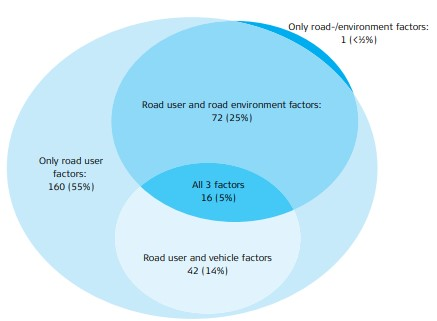
\includegraphics{accident_factors.jpg}
    \caption{Accident factors for investigated accidents\cite{danmark_why_accidents_happen_2014}}
    \label{fig:probana:accidentFactors}
\end{figure}
